\documentclass[tikz]{standalone}
\usetikzlibrary{positioning}
\newcommand{\red}[1]{\textcolor{red}{#1}}
\newcommand{\blue}[1]{\textcolor{blue}{#1}}
\newcommand{\teal}[1]{\textcolor{teal}{#1}}

\begin{document}
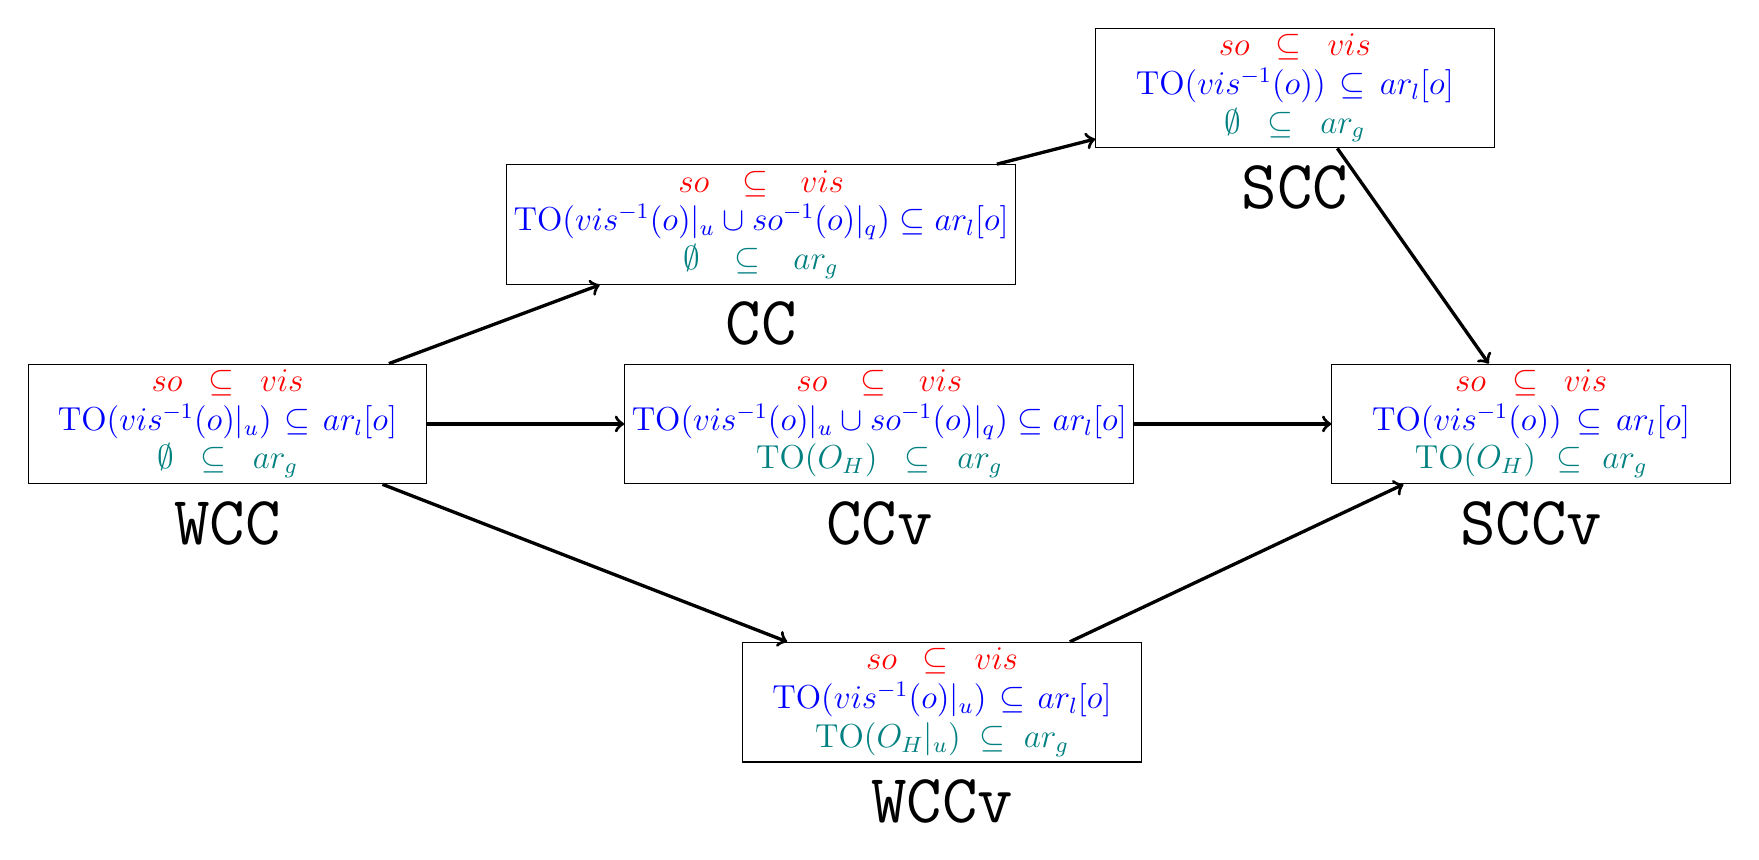
\begin{tikzpicture}
\tikzset{
  lconsistency/.style = {rectangle, fill=white, font=\large, draw, inner sep = 2pt, text width=18em, text centered},
  sconsistency/.style = {rectangle, fill=white, font=\large, draw, inner sep = 2pt, text width=14em, text centered},
  lemma/.style = {rectangle, rounded corners, fill=white, draw=white, line width = 1.5pt, inner sep = 6pt},
  po/.style = {->, very thick},
  cn/.style = {rectangle, fill=white, draw=white,font=\Huge},
}

  \node (wcc) [sconsistency] {%\Large WCC\\
                             \red{$so\subseteq vis$}\\
                             \blue{TO$(vis^{-1}(o)|_{u}) \subseteq ar_{l}[o]$}\\
                             \teal{$\emptyset \subseteq ar_g$}};
  \node (nwcc) [cn, below = 0.1cm of wcc] {\texttt{WCC}};

  \node (cc) [lconsistency, above right=1.0cm and 1.0cm of wcc] {%\large CC\\
                             \red{$so\subseteq vis$}\\
                            \blue{TO$(vis^{-1}(o)|_{u} \cup so^{-1}(o)|_{q})\subseteq ar_{l}[o]$}\\
                            \teal{$\emptyset \subseteq ar_g$}};
  \node (ncc) [cn, below = 0.1cm of cc] {\texttt{CC}};

  \node (scc) [sconsistency, above right = 0.2cm and 1.0cm of cc] {%\large SCC\\
                             \red{$so\subseteq vis$}\\
                            \blue{TO$(vis^{-1}(o))\subseteq ar_{l}[o]$}\\
                            \teal{$\emptyset \subseteq ar_g$}};
  \node (nscc) [cn, below = 0.1cm of scc] {\texttt{SCC}};

  \node (ccv) [lconsistency, right = 2.5cm of wcc] {%\large CCv\\
                             \red{$so\subseteq vis$}\\
                             \blue{TO$(vis^{-1}(o)|_{u} \cup so^{-1}(o)|_{q})\subseteq ar_{l}[o]$}\\
                             \teal{TO$(O_H)\subseteq ar_g$}};
  \node (nccv) [cn, below = 0.1cm of ccv] {\texttt{CCv}};

  \node (sccv) [sconsistency, right = 2.5cm of ccv] {%\large SCCv\\
                             \red{$so\subseteq vis$}\\
                            \blue{TO$(vis^{-1}(o))\subseteq ar_{l}[o]$}\\
                            \teal{TO$(O_H)\subseteq ar_g$}};
  \node (nsccv) [cn, below = 0.1cm of sccv] {\texttt{SCCv}};

  \node (wccv) [sconsistency, below right=2.0cm and 4.0cm of wcc] {%\large WCCv\\
                             \red{$so\subseteq vis$}\\
                             \blue{TO$(vis^{-1}(o)|_{u}) \subseteq ar_{l}[o]$}\\
                             \teal{TO$(O_H|_u)\subseteq ar_g$}};
  \node (nwccv) [cn, below = 0.1cm of wccv] {\texttt{WCCv}};

  \draw [po] (wcc) to (cc);
  \draw [po] (wcc) to (ccv);
  \draw [po] (cc) to (scc);
  \draw [po] (scc) to (sccv);
  \draw [po] (wcc) to (wccv);
  \draw [po] (ccv) to (sccv);
  \draw [po] (wccv) to (sccv);

\end{tikzpicture}
\end{document}
